\documentclass[11pt]{article}
\usepackage[margin=1in]{geometry}
\usepackage{xcolor,graphicx,booktabs,amsmath,hyperref,caption,microtype}
\hypersetup{colorlinks=true,linkcolor=blue!50!black,citecolor=blue!50!black,urlcolor=blue!50!black}
\captionsetup{font=small}
\graphicspath{{../results/figs/}}

\title{Beam, Wire, or Battery?\\[4pt]\large Valuing a Steerable Space Solar Power Beam with Real Hourly Electricity Prices}
\author{Kartikeya Goel\\Stanford University\\\texttt{kartgoel@stanford.edu}}
\date{October 2026 \quad (preprint, independent work)}

\begin{document}
\maketitle

\begin{abstract}
A geostationary (GEO) space-based solar power (SBSP) satellite can redirect its microwave beam between ground
rectennas within milliseconds. Advocates often cite this as a distinctive source of value, but it has not been
quantified with market data. We combine GEO visibility and rectenna-sizing geometry with 2024--2025 hourly
day-ahead prices from five U.S.\ markets (CAISO, ERCOT, MISO, NYISO, ISO-NE) and Spain (OMIE), and solve a
revenue-maximizing hourly beam allocation for a 2\,GW satellite. Steering raises energy revenue by 16--39\% over
the best single rectenna from a U.S.\ slot (100$^\circ$W) and by 22--36\% from a transatlantic slot (40$^\circ$W).
Two or three rectennas capture 70--94\% of the gain from using all of them. The gain is broad-based rather than spike-driven: the top 10\%
of hours supply about half of it. We then ask whether the same flexibility is cheaper to buy with a wire or a battery.
Between Spain and New England, a second rectenna roughly pays for itself at NASA's own ground-segment cost
(\$366M/yr added revenue against \$376M/yr annualized cost in 2025), while a 6,800\,km subsea HVDC line doing the
same job would cost about nine times more. Beyond about 900\,km over land or 300\,km subsea, a rectenna is a cheaper
``wire'' than HVDC. Over shorter distances, and in most cases on value per dollar, batteries or HVDC do better.
Price impact, which is large for a gigawatt-scale plant in a small market, roughly doubles the premium from the U.S.\ slot and leaves the transatlantic premium about unchanged.
Code and data are open.
\end{abstract}

\section{Introduction}
Space-based solar power, first proposed by Glaser~\cite{glaser1968}, has seen renewed attention with lower launch
costs and in-orbit demonstrations such as Caltech's SSPD-1~\cite{caltech2023}. Most economic assessments ask what a
kilowatt-hour costs~\cite{nasa2024,caltechjoule2025,niebla2025}. NASA's 2024 study found baseline costs of
\$0.61--1.59/kWh for its reference designs, competitive only if many favorable assumptions hold together~\cite{nasa2024}.

Cost per kWh treats SBSP as a generator fixed in place. Unlike any terrestrial plant, though, a GEO satellite can point
its output at any rectenna it can see, and electronically steered phased arrays can repoint in milliseconds.
Advocates describe this as ``a giant interconnector in space''~\cite{wef2025}, and recent techno-economic work names
``dynamic energy allocation'' between receivers as a key benefit~\cite{niebla2025}. Neither quantifies it.
The closest modeling work does not address it either. A European capacity-expansion study assumes a single satellite
feeds a dedicated ground station at every node simultaneously, inside a cost-minimizing central plan, with no price-driven
choice of where to deliver~\cite{che2025}. A recent LEO constellation study allocates power across eight ground
stations to meet demand, with no prices or revenue~\cite{leo2026}.

We ask three questions.
(i) Using real hourly prices, how much more does a GEO satellite earn by steering among rectennas in different markets
than by serving one?
(ii) How many rectennas is it worth building, given that each sits idle while the beam is elsewhere?
(iii) Is steering cheaper than the obvious alternatives, a long-distance HVDC line from a fixed rectenna or a battery at it?

\section{Methods}
\subsection{Geometry}
For a ground site at latitude $\phi$ and longitude $\lambda$ and a satellite at longitude $\lambda_s$, the central angle
$\gamma$ satisfies $\cos\gamma=\cos\phi\cos(\lambda-\lambda_s)$, elevation is
$\varepsilon=\arctan\!\big((\cos\gamma-R_E/r)/\sin\gamma\big)$ with $r=42{,}164$\,km, and slant range is
$d=\sqrt{r^2+R_E^2-2rR_E\cos\gamma}$. Because the diffraction-limited spot scales with $d$ and the footprint stretches by
$1/\sin\varepsilon$, we take rectenna area relative to a sub-satellite site as $A=(d/h)^2/\sin\varepsilon$, where
$h=35{,}786$\,km. Sites below 15$^\circ$ elevation are excluded. One-way atmospheric loss is 2\% at zenith, scaled
by airmass. Eclipses are computed minute by minute with a cylindrical Earth shadow. The satellite is unlit for
80\,h/yr (0.9\%), with a longest daily eclipse of 70\,min near the equinoxes.

We place one candidate rectenna on open land near each market's pricing hub (Table~\ref{tab:sites}).
Figure~\ref{fig:vis} shows elevation by slot. A U.S.\ slot at 100$^\circ$W sees all five U.S.\ sites at 33--53$^\circ$. A
transatlantic slot at 40$^\circ$W sees Spain, New England and New York at about 30$^\circ$ and Texas and Illinois
lower, but not California. No slot sees both California and Spain.

\begin{table}[h]\centering\small
\resizebox{\textwidth}{!}{\begin{tabular}{llrrrr}\toprule
Market & Price node & Site & Elev.\ 100$^\circ$W & Elev.\ 40$^\circ$W & 2025 mean \$/MWh\\\midrule
CAISO & SP15 hub & Mojave (35.0N, 117.5W) & 45.3 & 1.5 & 32.2\\
ERCOT & Hub average & W.\ Texas (31.5N, 100.0W) & 53.3 & 16.9 & 33.5\\
MISO & Illinois hub & C.\ Illinois (40.0N, 89.0W) & 42.3 & 22.1 & 38.7\\
NYISO & Capital zone & Upstate NY (42.7N, 74.5W) & 34.4 & 29.7 & 65.1\\
ISO-NE & Internal hub & C.\ Mass.\ (42.5N, 72.3W) & 33.5 & 31.1 & 67.8\\
OMIE & Spain & La Mancha (39.0N, 3.5W) & -- & 31.2 & 73.7\\\bottomrule
\end{tabular}}
\caption{Candidate rectenna sites. OMIE prices converted at 1.082 (2024) and 1.13 (2025) USD/EUR.}
\label{tab:sites}
\end{table}

\begin{figure}[t]\centering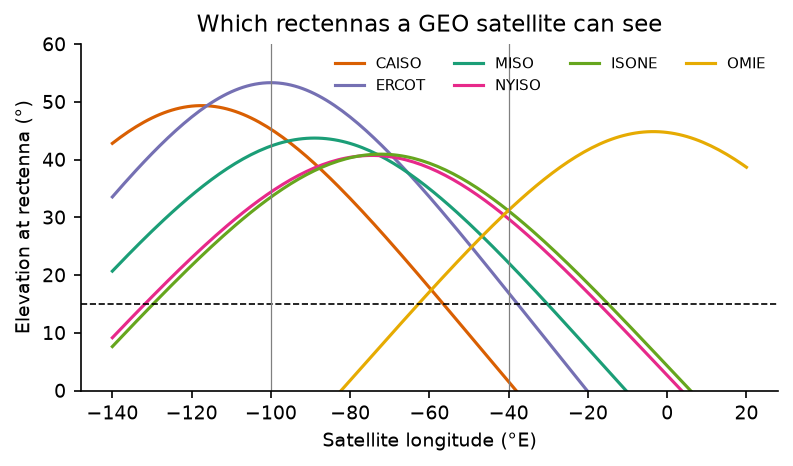
\includegraphics[width=0.75\textwidth]{fig1_visibility.png}
\caption{Rectenna elevation by GEO slot. Dashed line: 15$^\circ$ cutoff. Vertical lines: the two slots studied.}
\label{fig:vis}\end{figure}

\subsection{Prices and dispatch}
We use hourly day-ahead prices for calendar years 2024 and 2025, collected with the open-source \texttt{gridstatus}
library~\cite{gridstatus} and directly from ERCOT and OMIE~\cite{ercot,omie}. All are public and need no account.
Gaps of up to 3\,h are interpolated. Two OMIE days in 2025 were unavailable and are treated as rectenna outages.

The satellite delivers $P=2$\,GW (NASA RD1~\cite{nasa2024}) when sunlit. In each hour $t$ it chooses deliveries
$q_{it}\ge 0$ to rectennas $i$ in a chosen set $S$ to maximize
\begin{equation}
\textstyle\sum_{i\in S} q_{it}\,(p_{it}-k_i q_{it})\quad\text{s.t.}\quad \sum_i q_{it}/\eta_i \le P\,a_t,
\end{equation}
where $p_{it}$ is the price, $\eta_i$ the beam efficiency, $a_t$ the sunlit fraction, and $k_i$ a linear price-impact slope.
The beam can be split across rectennas (multi-beam phased array). The solution water-fills marginal revenue
$p_{it}-2k_iq_{it}$ at a common level $\lambda_t\ge 0$, so the satellite never sells at a negative margin. We set
$k_i=k_0\cdot(50\,\mathrm{GW}/L_i)$, scaling a reference slope $k_0$ by each market's average load $L_i$.
The main results use $k_0=0$ (price-taker), and we sweep $k_0\in[0,10]$\,\$/MWh per GW. The baseline is the
best single rectenna \emph{in hindsight}, which favors the fixed design. For every slot and year we evaluate all
subsets of visible rectennas.

\subsection{Costs and benchmarks}
NASA's 2024 study estimates a \$3.12B ground segment for RD1's single 6\,km, 2\,GW rectenna~\cite{nasa2024}. We take
this as the cost at a reference site of area factor $A=1.5$ (about 45$^\circ$ elevation) and scale linearly with $A$.
Capital is annualized at 7\% over 30 years (and at 3\% as a sensitivity). For the HVDC benchmark, a fixed rectenna
at the best site is joined by a 2\,GW line to the second site. We assume \$0.5B/GW for the converter pair, \$1.1M/km/GW
overland or \$3.3M/km/GW subsea, a 1.2 route factor, 1.5\% converter loss plus 3\% per 1,000\,km, and a 40-year life.
For the battery benchmark, a 2\,GW/8\,GWh battery (87\% round trip, \$250/kWh, 15 years) sits at the fixed site and
arbitrages day-ahead prices with perfect foresight (a linear program solved with HiGHS). All benchmarks are energy-only.

\section{Results}
\subsection{How much is steering worth?}
Figure~\ref{fig:prem} and Table~\ref{tab:main} show the premium over the best single rectenna. From 100$^\circ$W, steering
across all five U.S.\ sites adds 16.3\% (2025) and 38.6\% (2024). The difference reflects price levels. In 2025 New England
and New York were about twice as expensive as the other markets on average, leaving less to gain. In 2024 averages were
similar and hourly patterns, especially California's evening ramp, drove the gain. From 40$^\circ$W, Spain plus the U.S.\
East Coast adds 35.9\% (2025) and 21.5\% (2024). Spain and New England are six hours apart and peak at different
UTC times.

Returns diminish quickly. The second rectenna supplies 44--83\% of the total gain, and three rectennas reach at least 70\%
of it in every case. Scanning all slots (Fig.~\ref{fig:sweep}), the premium is about 16\% for slots that see only U.S.\ sites and jumps to
27--40\% for slots between 60$^\circ$W and 15$^\circ$W, where Spain and the U.S.\ East Coast are both in view.

\begin{table}[h]\centering\small
\resizebox{\textwidth}{!}{\begin{tabular}{lrrrr}\toprule
 & US 2025 & US 2024 & Atlantic 2025 & Atlantic 2024\\\midrule
Best single site (\$M/yr) & ISO-NE 1,139 & ISO-NE 698 & Spain 1,227 & Spain 1,145\\
+ 2nd site & +7.1\% (NYISO) & +21.1\% (CAISO) & +29.8\% (ISO-NE) & +13.6\% (ISO-NE)\\
+ 3rd site & +11.5\% & +34.6\% & +33.3\% & +20.1\% \\
All visible & +16.3\% & +38.6\% & +35.9\% & +21.5\%\\
Share of gain in top 10\% of hours & 49\% & 57\% & 48\% & 64\%\\
Break-even 2nd rectenna cost, 7\% / 3\% (\$B) & 0.74 / 1.18 & 1.78 / 2.82 & 3.04 / 4.79 & 1.29 / 2.04\\\bottomrule
\end{tabular}}
\caption{Steering premium over the best single rectenna ($k_0=0$). NASA's estimate is \$3.12B per site.}
\label{tab:main}
\end{table}

\begin{figure}[t]\centering
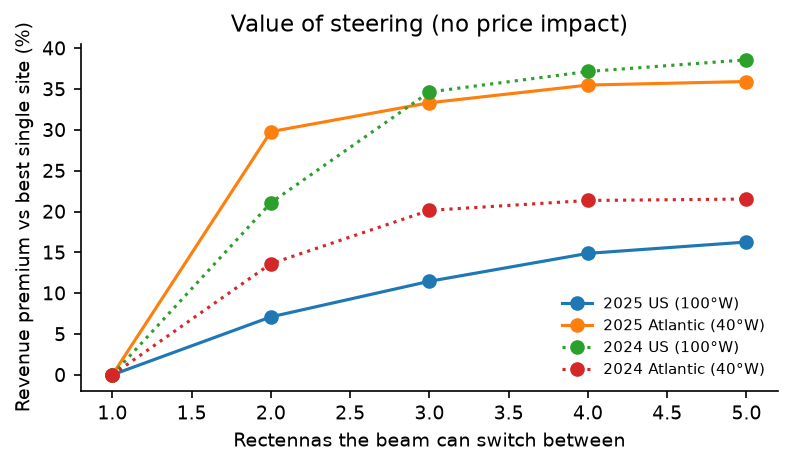
\includegraphics[width=0.49\textwidth]{fig2_premium_by_n.png}\hfill
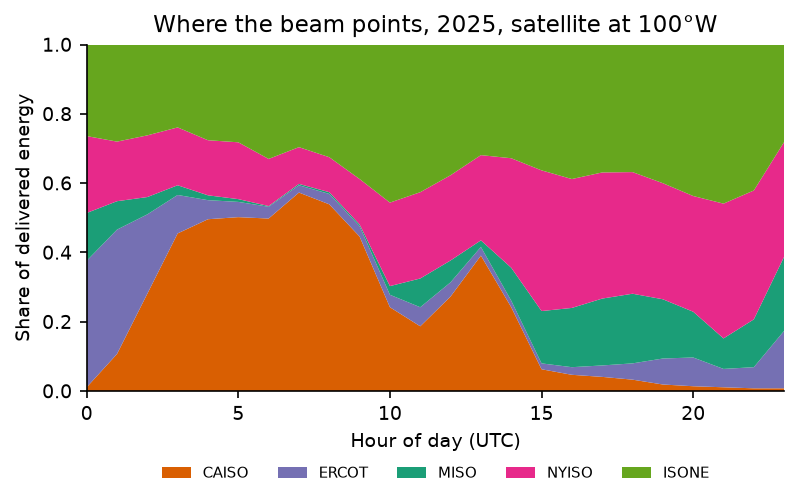
\includegraphics[width=0.49\textwidth]{fig4_beam_share_by_hour.png}
\caption{Left: premium by number of rectennas (best subset at each size). Right: where the beam points by UTC hour,
2025, 100$^\circ$W. California dominates its evening (02--09 UTC). The Northeast takes the rest.}
\label{fig:prem}\end{figure}

\subsection{Is the value in spikes?}
We expected most of the gain to come from rare scarcity events such as ERCOT's \$2,221/MWh hour in 2024. It does not.
The top 1\% of hours supply 10--27\% of the gain and the top 10\% supply 48--64\%. The beam earns most of its premium
from ordinary daily patterns, solar-driven midday troughs in California and Spain and evening peaks at different UTC
times, on 3,200--6,400 hours a year. This makes the result more robust to which year is studied than a spike-driven
gain would be. It also means the gain could shrink as storage flattens daily price shapes.

\subsection{Price impact}
A 2\,GW injection is large relative to New England (13\,GW average load) or New York (17\,GW). With price impact on, a
single-site satellite depresses its own price, and spreading output across markets avoids that. The premium therefore rises
with $k_0$ (Fig.~\ref{fig:impact}). In the U.S.\ slot it rises from 16\% to 32\% at $k_0=2$ and to 62\% at $k_0=5$. The
transatlantic premium is less sensitive, because Spain is larger: with all stations it edges up (36\% to 41\% at $k_0=5$),
but the two-station Spain--New England premium falls (30\% to 24\%), because New England's small market saturates. We regard $k_0\approx1$--2 as plausible but uncertain. The
qualitative conclusion is that price impact is a reason to steer among several small markets, not a limit on it, but
it penalizes leaning on one small market.

\begin{figure}[t]\centering
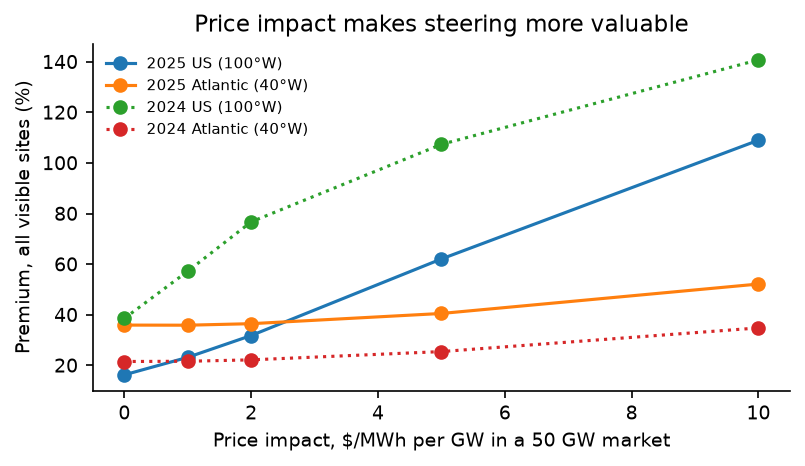
\includegraphics[width=0.49\textwidth]{fig5_price_impact.png}\hfill
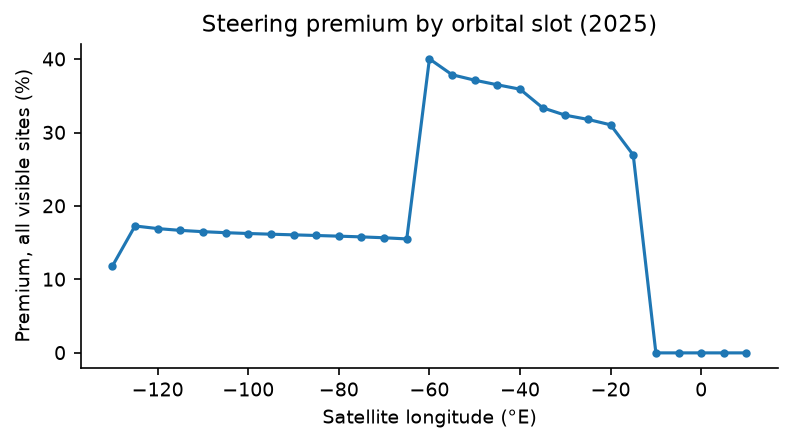
\includegraphics[width=0.49\textwidth]{fig7_slot_sweep.png}
\caption{Left: premium versus price-impact slope. Right: premium by GEO slot, 2025. The step at 60$^\circ$W is Spain entering view. East of 15$^\circ$W only Spain is visible.}
\label{fig:impact}\label{fig:sweep}\end{figure}

\subsection{Beam, wire, or battery?}
Figure~\ref{fig:bench} compares the added revenue of each option to its annualized cost. Three patterns stand out.

\emph{Over long distances, the beam is the cheapest wire.} Between Spain and New England (2025), a second rectenna adds
\$366M/yr at an annualized cost of \$376M/yr (ratio 0.97), essentially break-even at NASA's cost and comfortably
positive at a 3\% discount rate (break-even \$4.79B). The equivalent subsea HVDC line (6,775\,km, 22\% losses) would
add only \$226M/yr at about \$3.43B/yr. For a 2\,GW line, the rectenna is cheaper than HVDC beyond about 890\,km overland or
300\,km subsea.

\emph{Over short distances, it is not.} The best U.S.\ pair in 2025 is New England--New York, 218\,km apart. There an HVDC
line (ratio 0.62) beats a second rectenna (0.24).

\emph{Batteries often win on value per dollar.} A co-located 2\,GW/8\,GWh battery achieves ratios of 0.35--1.22, best in Spain,
whose midday solar trough creates large daily spreads. Batteries and steering capture overlapping but distinct value (time
shifting versus place shifting) and are complements, not substitutes.

Inside the U.S., a second rectenna would need to cost \$0.7--1.8B, 24--57\% of NASA's estimate, to pay for itself.

\begin{figure}[t]\centering
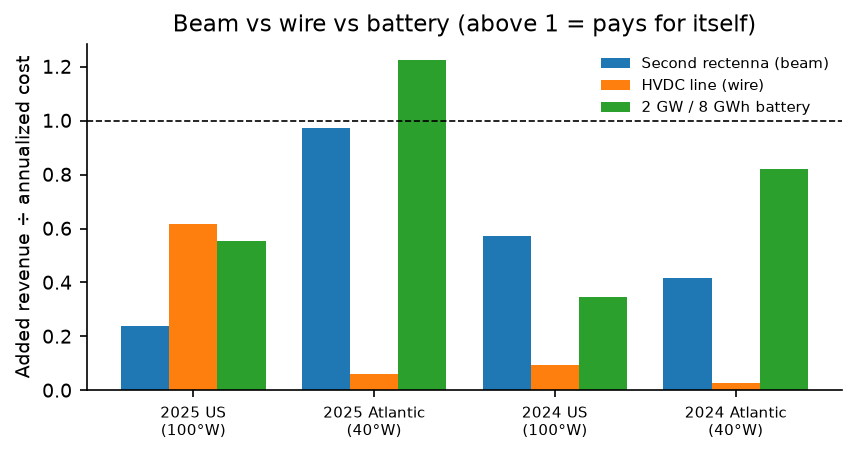
\includegraphics[width=0.49\textwidth]{fig3_benchmarks.png}\hfill
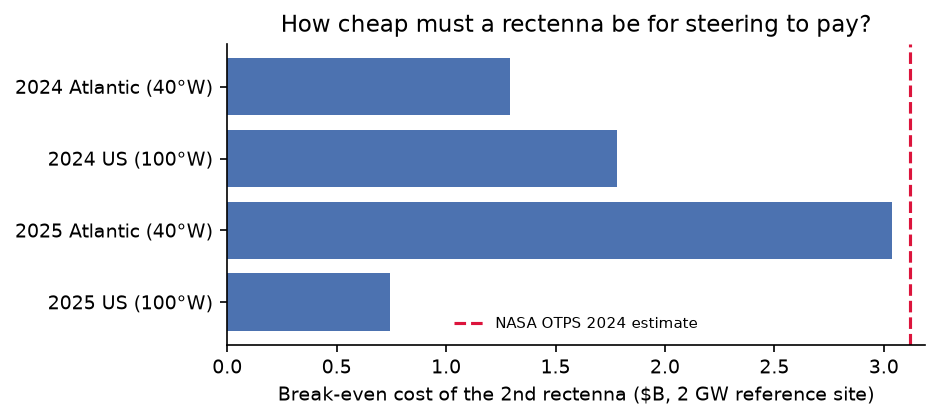
\includegraphics[width=0.49\textwidth]{fig6_breakeven.png}
\caption{Left: added revenue divided by annualized cost; above 1 pays for itself. Right: break-even cost of the second
rectenna versus NASA's estimate.}
\label{fig:bench}\end{figure}

\section{Discussion and limitations}
Steering is real value, with a 16--39\% revenue premium, but it does not rescue SBSP economics. NASA's baseline costs are an
order of magnitude above wholesale prices~\cite{nasa2024}, and a 20--40\% revenue gain does not close that gap. What steering
changes is \emph{system design}. Designers should plan for two or three rectennas, chosen to pair markets in distant time
zones rather than neighbors. The transatlantic slot is the most attractive we found. A satellite serving both continents could
be viewed as a 2\,GW intercontinental interconnector whose ``line'' costs one rectenna.

The analysis is deliberately simple. (1) Prices are day-ahead and energy-only. Real-time spikes, capacity and ancillary
revenues would add value to all options. (2) Two years is a short record. (3) Rectenna costs are highly uncertain and we
scale a single NASA estimate. (4) The HVDC line can also carry other generators' power when the satellite is not using it,
which we do not credit. (5) Price impact is linear and static, and future markets with more storage and solar will differ.
(6) We ignore regulatory and siting barriers to cross-border delivery, which may dominate for the transatlantic case.
(7) Hub prices understate congestion near rectenna sites. Extensions include multi-satellite fleets sharing rectennas,
real-time markets, and co-optimizing steering with storage.

\section{Conclusion}
Using real prices from six markets, a GEO satellite that steers among two or three well-chosen rectennas earns 16--39\% more
than one serving a single site. Across the Atlantic, the second rectenna roughly pays for itself at NASA's cost and is about
nine times cheaper than the equivalent subsea HVDC line. The ``interconnector in space'' claim holds over long distances.
Over short ones it is beaten by wires and batteries.

\paragraph{Code and data.} \url{https://github.com/KartikeyaGoel/sbsp-beam-steering}

\paragraph{Acknowledgment.} Analysis and drafting were assisted by an AI model (Claude, Anthropic). The author is
responsible for all content.

\begin{thebibliography}{99}\small
\bibitem{glaser1968} P.~E. Glaser, ``Power from the Sun: Its future,'' \emph{Science} 162(3856):857--861, 1968.
\bibitem{caltech2023} Caltech, ``Space Solar Power Project ends first in-space mission with successes and lessons,'' 2024.
\url{https://www.caltech.edu/about/news/space-solar-power-project-ends-first-in-space-mission-with-successes-and-lessons}
\bibitem{nasa2024} E.~Rodgers et al., ``Space-Based Solar Power,'' NASA Office of Technology, Policy, and Strategy, Jan.\ 2024.
\bibitem{caltechjoule2025} ``Space solar power generation: A viable system proposal and technoeconomic analysis,'' \emph{Joule}, 2025.
\bibitem{niebla2025} M.~T. Niebla del Campo, O.~Karasu, M.~Riede, ``An economic impact analysis for space-based solar power systems on the world's economy,'' IAC-25-E6.IP.3x100979, 2025.
\bibitem{wef2025} World Economic Forum, ``Why we need space-based solar power,'' Oct.\ 2025.
\bibitem{che2025} Che, He, and Liu, ``Assess space-based solar power for European-scale power system decarbonization,'' \emph{Joule}, 2025; arXiv:2504.05052.
\bibitem{leo2026} ``Constellation-level power allocation for LEO space-based solar power,'' arXiv:2606.18416, 2026.
\bibitem{gridstatus} Grid Status, \texttt{gridstatus} Python library v0.36. \url{https://github.com/gridstatus/gridstatus}
\bibitem{ercot} ERCOT, ``Historical DAM Load Zone and Hub Prices'' (report 13060).
\bibitem{omie} OMIE, day-ahead marginal price files (\texttt{marginalpdbc}).
\end{thebibliography}
\end{document}
